\chapter{Verzamelingen}
\label{chap:verzamelingen}
%%%%% vullen in kleuren bij venn
%\def\vuleen{\fill[red, opacity=0.3]}
%\def\vultwee{\fill[green, opacity=0.3]}
\def\vulgrijs{\fill[black!30,opacity=0.5]}

%%%%% vullen met arceringen bij venn
\def\vuleen{\fill[pattern=horizontal lines,pattern color=blue]}
\def\vultwee{\fill[pattern=vertical lines,pattern color=red]}
\def\arceerschuin{\fill[pattern=north east lines,pattern color=blue]}
\def\arceerpuntjes{\fill[pattern=dots,pattern color=blue]}

% Definition of circles
\def\firstcircle{(0,0) ellipse [x radius=1.5cm, y radius=2cm]}
\def\secondcircle{(0:2cm) ellipse [x radius=1.5cm, y radius=2cm]}
\def\tweedecirkel{(0:1.5cm) ellipse [x radius=1.5cm, y radius=2cm]}

\def\firstellipse{(40:1.55cm) ellipse [x radius=2cm,y radius=1.5cm]}
  \def\secondellipse{(140:1.5cm) ellipse [x radius=2cm,y radius=1.5cm]}
  \def\thirdellipse{(270:0.5cm) ellipse [x radius=2cm,y radius=1.5cm]}

%2 verticale ellipsen
\def\vertellipl{(0,0) ellipse [x radius=1cm, y radius=2cm]}
\def\vertellipr{(3,0) ellipse [x radius=1cm, y radius=2cm]}

%2 grotere verticale ellipsen
\def\grvertellipl{(0,0) ellipse [x radius=1.5cm, y radius=3cm]}
\def\grvertellipr{(4,0) ellipse [x radius=1.5cm, y radius=3cm]}

% bolletje voor elementen
\def\bol{circle (1.5pt)}

\colorlet{circle edge}{black!70}
\colorlet{circle area}{blue!20}

\tikzset{filled/.style={fill=circle area, draw=circle edge, thick},
    outline/.style={draw=circle edge, thick}}
    
\begin{tikzpicture}[thick]
\draw \vertellipl node [above=2.3cm, left] {$A$};
\draw \vertellipr node [above=2.3cm, left] {$B$};
% linkse elementen
\draw[fill] (0,1.3) \bol node [above] {1};
\draw[fill] (0,0.4) \bol node [above] {2};
\draw[fill] (0,-0.5) \bol node [above] {3};
\draw[fill] (0,-1.4) \bol node [above] {4};
% rechtse elementen
\draw[fill] (3,1.3) \bol node [above] {4};
\draw[fill] (3,0.4) \bol node [above] {5};
\draw[fill] (3,-0.5) \bol node [above] {6};
\draw[fill] (3,-1.4) \bol node [above] {7};
% pijlen
\begin{scope}[decoration={
    markings,
    mark=at position 0.5 with {\arrow{>}}}
    ] 
    \draw[postaction={decorate}] (0,1.3) to (3,1.3);
    \draw[postaction={decorate}] (0,0.4) to (3,0.4);
    \draw[postaction={decorate}] (0,-0.5) to (3,-0.5);
    \draw[postaction={decorate}] (0,-1.4) to (3,-1.4);
\end{scope}
\end{tikzpicture}

% Figuur domein en bereik
\begin{tikzpicture}[thick]
\draw \vertellipl node [above=2.3cm, left] {$A$};
\draw \vertellipr node [above=2.3cm, left] {$B$};
% linkse elementen
\draw[fill] (0,1.3) \bol node [above] {1};
\draw[fill] (0,0.4) \bol node [above] {2};
\draw[fill] (0,-0.5) \bol node [above] {3};
\draw[fill] (0,-1.4) \bol node [above] {4};
% rechtse elementen
\draw[fill] (3,1) \bol node [above] {a};
\draw[fill] (3,0) \bol node [above] {b};
\draw[fill] (3,-1) \bol node [above] {c};
% pijlen
\begin{scope}[decoration={
    markings,
    mark=at position 0.5 with {\arrow{>}}}
    ] 
    \draw[postaction={decorate}] (0,1.3) to (3,1);
    \draw[postaction={decorate}] (0,1.3) to (3,0);
    \draw[postaction={decorate}] (0,0.4) to (3,0);
    \draw[postaction={decorate}] (0,-1.4) to (3,0);
\end{scope}
\end{tikzpicture}



% Figuur veel-op-een relatie voorbeeld 1 (y=x^2)
\begin{tikzpicture}[thick]
\draw \grvertellipl node [above=3.3cm, left] {$A$};
\draw \grvertellipr node [above=3.3cm, left] {$B$};
% linkse elementen
\draw[fill] (0,2.2) \bol node [above] {$-3$};
\draw[fill] (0,1.3) \bol node [above] {$-2$};
\draw[fill] (0,0.4) \bol node [above] {$-1$};
\draw[fill] (0,-0.5) \bol node [above] {$1$};
\draw[fill] (0,-1.4) \bol node [above] {$2$};
\draw[fill] (0,-2.3) \bol node [above] {$3$};
% rechtse elementen
\draw[fill] (4,2.3) \bol node [above] {$1$};
\draw[fill] (4,1.4) \bol node [above] {$2$};
\draw[fill] (4,0.5) \bol node [above] {$4$};
\draw[fill] (4,-0.4) \bol node [above] {$5$};
\draw[fill] (4,-1.3) \bol node [above] {$8$};
\draw[fill] (4,-2.2) \bol node [above] {$9$};
% pijlen
\begin{scope}[decoration={
    markings,
    mark=at position 0.5 with {\arrow{>}}}
    ] 
    \draw[postaction={decorate}] (0,2.2) to (4,-2.2);
    \draw[postaction={decorate}] (0,1.3) to (4,0.5);
    \draw[postaction={decorate}] (0,0.4) to (4,2.3);
    \draw[postaction={decorate}] (0,-0.5) to (4,2.3);
    \draw[postaction={decorate}] (0,-1.4) to (4,0.5);
    \draw[postaction={decorate}] (0,-2.3) to (4,-2.2);
\end{scope}
\end{tikzpicture}


% Figuur een-op-een relatie def algemeen
\begin{tikzpicture}[thick]
\draw \grvertellipl node [above=3.3cm, left] {$A$};
\draw \grvertellipr node [above=3.3cm, left] {$B$};
% linkse elementen
\draw[fill] (0,2.2) \bol node [above] {$x_1$};
\draw[fill] (0,1.3) \bol node [above] {$x_2$};
\draw[fill] (0,0.4) \bol node [above] {$x_3$};
\draw[fill] (0,-0.5) \bol node [above] {$x_4$};
\draw[fill] (0,-1.4) \bol node [above] {$x_5$};
\draw[fill] (0,-2.3) \bol node [above] {$x_6$};
% rechtse elementen
\draw[fill] (4,2.3) \bol node [above] {$y_1$};
\draw[fill] (4,1.4) \bol node [above] {$y_2$};
\draw[fill] (4,0.5) \bol node [above] {$y_3$};
\draw[fill] (4,-0.4) \bol node [above] {$y_4$};
\draw[fill] (4,-1.3) \bol node [above] {$y_5$};
\draw[fill] (4,-2.2) \bol node [above] {$y_6$};
% pijlen
\begin{scope}[decoration={
    markings,
    mark=at position 0.5 with {\arrow{>}}}
    ] 
    \draw[postaction={decorate}] (0,2.2) to (4,-2.2);
    \draw[postaction={decorate}] (0,1.3) to (4,0.5);
    \draw[postaction={decorate}] (0,0.4) to (4,2.3);
    \draw[postaction={decorate}] (0,-0.5) to (4,-0.4);
    \draw[postaction={decorate}] (0,-1.4) to (4,-1.3);
    \draw[postaction={decorate}] (0,-2.3) to (4,1.4);
\end{scope}
\end{tikzpicture}

% Prijs van schoenen i.f.v. aantal
\begin{figure}[htbp]
    \centering
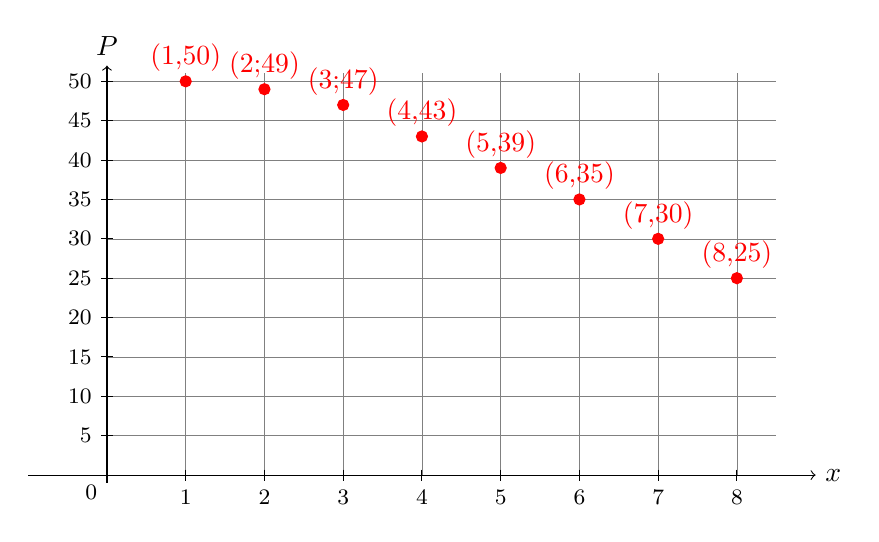
\begin{tikzpicture}[x=1cm,y=0.1cm]
\draw[help lines] (0,0) grid [xstep=1, ystep=5] (8.5,51);
\draw[->] (-1,0) -- (9,0) node[right] {$x$};
\draw[->] (0,-1) -- (0,52) node[above] {$P$};
\foreach \x in {1,...,8}
	\draw[shift={(\x,0)}] (0pt,2pt) -- (0pt,-2pt) node[below] {\footnotesize $\x$};
\foreach \y in {5,10,...,50}
	\draw[shift={(0,\y)},color=black] (2pt,0pt) -- (-2pt,0pt) node[left] {\footnotesize $\y$};
\node [below left] at (0,0) {\footnotesize 0};
\filldraw [red] (1,50) circle (2pt) node[above] {(1,50)};
\filldraw [red] (2,49) circle (2pt) node[above] {(2;49)};
\filldraw [red] (3,47) circle (2pt) node[above] {(3;47)};
\filldraw [red] (4,43) circle (2pt) node[above] {(4,43)};
\filldraw [red] (5,39) circle (2pt) node[above] {(5,39)};
\filldraw [red] (6,35) circle (2pt) node[above] {(6,35)};
\filldraw [red] (7,30) circle (2pt) node[above] {(7,30)};
\filldraw [red] (8,25) circle (2pt) node[above] {(8,25)};
\end{tikzpicture}
\caption{Prijs $P(x)$}
    \label{fig:taxirechte}
\end{figure}

%%getallen kleiner dan 10
%\begin{tikzpicture}
%\draw[outline] (0,0) ellipse [x radius=1.5cm, y radius=2cm] node at (1,2) {$A$};
%\draw[fill] (0.7,0.8) circle (0.4mm) node[above] {$1$};
%\draw[fill] (-0.6,0.9) circle (0.4mm) node[above] {$2$};
%\draw[fill] (0,1) circle (0.4mm) node[above] {$3$};
%\draw[fill] (0.3,0.2) circle (0.4mm) node[above] {$4$};
%\draw[fill] (-0.9,0.2) circle (0.4mm) node[above] {$5$};
%\draw[fill] (-0.9,-0.9) circle (0.4mm) node[above] {$6$};
%\draw[fill] (0.4,-.7) circle (0.4mm) node[above] {$7$};
%\draw[fill] (1.1,-0.8) circle (0.4mm) node[above] {$8$};
%\draw[fill] (0,-1.3) circle (0.4mm) node[above] {$9$};
%\end{tikzpicture}
%
%%regenboogkleuren
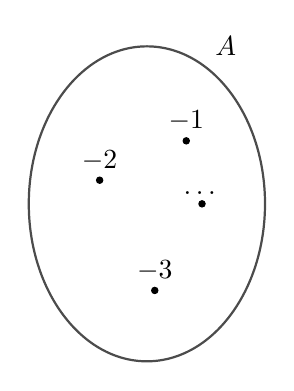
\begin{tikzpicture}
\draw[outline] (0,0) ellipse [x radius=1.5cm, y radius=2cm] node at (1,2) {$A$};
\draw[fill] (0.5,0.8) circle (0.4mm) node[above] {$-1$};
\draw[fill] (-0.6,0.3) circle (0.4mm) node[above] {$-2$};
\draw[fill] (0.7,0) circle (0.4mm) node[above] {\ldots};
\draw[fill] (0.1,-1.1) circle (0.4mm) node[above] {$-3$};
\end{tikzpicture}
%
%%conjuncte verzamelingen
%\begin{tikzpicture}
%    \draw[outline] \firstcircle node at (-0.5,2.2) {$A$};
%    \draw[outline] \tweedecirkel node at (1.7,2.2) {$B$};
%    \draw[fill] (-0.9,0) circle (0.4mm) node[above] {$a$};
%    \draw[fill] (0.7,0.6) circle (0.4mm) node[above] {$b$};
%    \draw[fill] (0.6,-0.9) circle (0.4mm) node[above] {$c$};
%    \draw[fill] (2,0.3) circle (0.4mm) node[above] {$d$};
%\end{tikzpicture}
%
%%disjuncte verzamelingen
%\begin{tikzpicture}
%    \draw[outline] \firstcircle node at (-0.5,2.2) {$A$};
%    \draw[outline] \tweedecirkel node at (1.7,2.2) {$B$};
%    \draw[fill] (-0.9,0) circle (0.4mm) node[above] {$a$};
%    \draw[fill] (-0.7,0.9) circle (0.4mm) node[above] {$b$};
%    \draw[fill] (-0.6,-0.9) circle (0.4mm) node[above] {$c$};
%    \draw[fill] (2,0.7) circle (0.4mm) node[above] {$d$};
%    \draw[fill] (2.1,-0.1) circle (0.4mm) node[above] {$e$};
%    \draw[fill] (1.8,-0.9) circle (0.4mm) node[above] {$f$};
%\end{tikzpicture}
%
%% Set A and B
%\begin{tikzpicture}
%    \begin{scope}
%        \clip \firstcircle;
%        \fill[filled] \secondcircle;
%    \end{scope}
%    \draw[outline] \firstcircle node {$A$};
%    \draw[outline] \secondcircle node {$B$};
%    \node[anchor=south] at (current bounding box.north) {$A \cap B$};
%\end{tikzpicture}
%
%%Set A or B but not (A and B) also known a A xor B
%\begin{tikzpicture}
%    \draw[filled, even odd rule] \firstcircle node {$A$}
%                                 \secondcircle node{$B$};
%    \node[anchor=south] at (current bounding box.north) {$\overline{A \cap B}$};
%\end{tikzpicture}
%
%% Set A or B
%\begin{tikzpicture}
%    \draw[filled] \firstcircle node {$A$}
%                  \secondcircle node {$B$};
%    \node[anchor=south] at (current bounding box.north) {$A \cup B$};
%\end{tikzpicture}
%
%% Set A but not B
%\begin{tikzpicture}
%    \begin{scope}
%        \clip \firstcircle;
%        \draw[filled, even odd rule] \firstcircle node {$A$}
%                                     \secondcircle;
%    \end{scope}
%    \draw[outline] \firstcircle
%                   \secondcircle node {$B$};
%    \node[anchor=south] at (current bounding box.north) {$A - B$};
%\end{tikzpicture}
%
%% Set B but not A
%\begin{tikzpicture}
%    \begin{scope}
%        \clip \secondcircle;
%        \draw[filled, even odd rule] \firstcircle
%                                     \secondcircle node {$B$};
%    \end{scope}
%    \draw[outline] \firstcircle node {$A$}
%                   \secondcircle;
%    \node[anchor=south] at (current bounding box.north) {$B - A$};
%\end{tikzpicture}
%
\def\firstellipse{(40:1.55cm) ellipse [x radius=2cm,y radius=1.5cm]}
  \def\secondellipse{(140:1.5cm) ellipse [x radius=2cm,y radius=1.5cm]}
  \def\thirdellipse{(270:0.5cm) ellipse [x radius=2cm,y radius=1.5cm]}
%\begin{tikzpicture}
%\fill[pattern=dots] \firstellipse;
%      \begin{scope}
%    \clip \secondellipse;
%    \fill[pattern=vertical lines] \thirdellipse;
%      \end{scope}
%%      \begin{scope}
%%    \clip \firstellipse;
%%    \fill[cyan] \thirdellipse;
%%      \end{scope}
%
%      \draw \firstellipse node at (30:4cm) {$A$};
%      \draw \secondellipse node at (150:4cm) {$B$};
%      \draw \thirdellipse node at (270:3cm) {$C$};
%    \end{tikzpicture}
%  %Zelfde met kleuren en transparantie  
%    \begin{tikzpicture}[thick]
%\fill[red, opacity=0.5] \firstellipse;
%      \begin{scope}
%    \clip \secondellipse;
%    \fill[green, opacity=0.5] \thirdellipse;
%      \end{scope}
%%      \begin{scope}
%%    \clip \firstellipse;
%%    \fill[cyan] \thirdellipse;
%%      \end{scope}
%
%      \draw \firstellipse node at (35:3.7cm) {$A$};
%      \draw \secondellipse node at (145:3.7cm) {$B$};
%      \draw \thirdellipse node at (270:2.7cm) {$C$};
%    \end{tikzpicture}
%    
%      %Zelfde met kleuren en transparantie, versie 3 
%    \begin{tikzpicture}[thick]
%\fill[black!40, opacity=0.5] \firstellipse;
%      \begin{scope}
%    \clip \secondellipse;
%    \fill[black!60, opacity=0.5] \thirdellipse;
%      \end{scope}
%%      \begin{scope}
%%    \clip \firstellipse;
%%    \fill[cyan] \thirdellipse;
%%      \end{scope}
%
%      \draw \firstellipse node at (35:3.7cm) {$A$};
%      \draw \secondellipse node at (145:3.7cm) {$B$};
%      \draw \thirdellipse node at (270:2.4cm) {$C$};
%    \end{tikzpicture}
%    
%          %Zelfde met arceringen en transparantie, versie 4 
%    \begin{tikzpicture}[thick]
%\vuleen \firstellipse;
%      \begin{scope}
%    \clip \secondellipse;
%    \vultwee \thirdellipse;
%      \end{scope}
%%      \begin{scope}
%%    \clip \firstellipse;
%%    \fill[cyan] \thirdellipse;
%%      \end{scope}
%
%      \draw \firstellipse node at (35:3.7cm) {$A$};
%      \draw \secondellipse node at (145:3.7cm) {$B$};
%      \draw \thirdellipse node at (270:2.3cm) {$C$};
%    \end{tikzpicture}
%    
%  
%  %%% (A u B) n (A u C)
%            %Zelfde met arceringen en transparantie, versie 4 
%    \begin{tikzpicture}[thick]
%\vuleen \firstellipse;
%\vuleen \secondellipse;
%\vultwee \firstellipse;
%\vultwee \thirdellipse;
%%      \begin{scope}
%%    \clip \firstellipse;
%%    \fill[cyan] \thirdellipse;
%%      \end{scope}
%
%      \draw \firstellipse node at (35:3.7cm) {$A$};
%      \draw \secondellipse node at (145:3.7cm) {$B$};
%      \draw \thirdellipse node at (270:2.3cm) {$C$};
%    \end{tikzpicture}  

%unie algemeen
\begin{tikzpicture}[thick]
\vuleen \firstellipse;
\vuleen \secondellipse;
%\vultwee \firstellipse;
%\vultwee \thirdellipse;
%      \begin{scope}
%    \clip \firstellipse;
%    \fill[cyan] \thirdellipse;
%      \end{scope}

 \draw \firstellipse node at (35:3.7cm) {$A$};
 \draw \secondellipse node at (145:3.7cm) {$B$};
 %     \draw \thirdellipse node at (270:2.3cm) {$C$};
    \end{tikzpicture} 
    
%%unievoorbeeld
%\begin{tikzpicture}[thick]
%\draw \firstellipse node at (35:3.7cm) {$Y$};
%\draw \secondellipse node at (145:3.7cm) {$X$};
%%\vulgrijs \firstellipse;
%%\vulgrijs \secondellipse;
%\draw[fill] (-2,1.4) \bol node [above] {a};
%\draw[fill] (-1.7,0.6) \bol node [above] {b};
%\draw[fill] (0,1) \bol node [above] {c};
%\draw[fill] (2,1.4) \bol node [above] {d};
%\draw[fill] (1.7,0.5) \bol node [above] {e};
%\end{tikzpicture}  
%
%%doorsnede algemeen
%\begin{tikzpicture}[thick]
%\begin{scope}
%    \clip \firstellipse;
%    \arceerschuin \secondellipse;
%\end{scope}
%\draw \firstellipse node at (35:3.7cm) {$A$};
%\draw \secondellipse node at (145:3.7cm) {$B$};
%    \end{tikzpicture} 
%    
%%doorsnedevoorbeeld
%\begin{tikzpicture}[thick]
%\draw \firstellipse node at (35:3.7cm) {$Y$};
%\draw \secondellipse node at (145:3.7cm) {$X$};
%\begin{scope}
%    \clip \firstellipse;
%    \arceerpuntjes \secondellipse;
%\end{scope}
%\draw[fill] (-1.5,1.6) \bol node [above] {1};
%\draw[fill] (-2.3,1.4) \bol node [above] {2};
%\draw[fill] (-1.2,1) \bol node [above] {3};
%\draw[fill] (-1.3,0) \bol node [above] {4};
%\draw[fill] (-2,0.7) \bol node [above] {5};
%\draw[fill] (0,1.4) \bol node [above] {6};
%\draw[fill] (-0.4,1) \bol node [above] {7};
%\draw[fill] (0.3,0.5) \bol node [above] {8};
%\draw[fill] (1.5,1.7) \bol node [above] {9};
%\draw[fill] (2,1) \bol node [above] {10};
%\draw[fill] (1.7,0.3) \bol node [above] {\ldots};
%\end{tikzpicture} 
%
%%verschil algemeen: A - B
%\begin{tikzpicture}[thick]
%    \begin{scope}
%        \clip \firstellipse;
%        \draw[pattern=north east lines,pattern color=blue, even odd rule] \firstellipse node{} \secondellipse;
%    \end{scope}
%\draw \firstellipse node at (35:3.7cm) {$A$};
%\draw \secondellipse node at (145:3.7cm) {$B$};
%    \end{tikzpicture} 
%    
%%verschil voorbeeld
%\begin{tikzpicture}[thick]
%    \begin{scope}
%        \clip \secondellipse;
%        \draw[pattern=dots,pattern color=blue, even odd rule] \firstellipse node{} \secondellipse;
%    \end{scope}
%\draw \firstellipse node at (35:3.7cm) {$A$};
%\draw \secondellipse node at (145:3.7cm) {$B$};
%\draw[fill] (-1.5,1.6) \bol node [above] {1};
%\draw[fill] (-1.7,0.5) \bol node [above] {2};
%\draw[fill] (0,1.4) \bol node [above] {3};
%\draw[fill] (0,0.3) \bol node [above] {4};
%\draw[fill] (2,0.8) \bol node [above] {5}; 
%    \end{tikzpicture} 
%    
%    
%%Complement algemeen
%\begin{tikzpicture}[thick]
%\draw[pattern=north east lines,pattern color=blue] (-1.5,-1) rectangle (4,3) node [above] {$U$};
%\fill[white] \firstellipse;
%\draw \firstellipse node at (35:3.7cm) {$A$};
%\end{tikzpicture} 
%    
%    
%%Complement voorbeeld
%\begin{tikzpicture}[thick]
%\draw[pattern=dots,pattern color=blue] (-1.5,-1) rectangle (4,3) node [above] {$U$};
%\fill[white] \firstellipse;
%\draw \firstellipse node at (35:3.7cm) {$A$};
%\draw[fill] (-1,2.3) \bol node [above] {0};
%\draw[fill] (-0.2,2.5) \bol node [above] {1};
%\draw[fill] (-1.1,1.4) \bol node [above] {2};
%\draw[fill] (-1.2,-0.4) \bol node [above] {\ldots};
%\draw[fill] (3,-0.5) \bol node [above] {98};
%\draw[fill] (3.5,0.8) \bol node [above] {99};
%\draw[fill] (1,1.8) \bol node [above] {100};
%\draw[fill] (0,0.5) \bol node [above] {101};
%\draw[fill] (2,0) \bol node [above] {102};
%\draw[fill] (2.3,1.2) \bol node [above] {\ldots};          
%\end{tikzpicture} 
%
%
%\begin{tikzpicture}[scale=0.7,thick]
%%\vuleen \firstellipse;
%\begin{scope}
%    \clip \firstellipse;
%    \vuleen \thirdellipse;
%\end{scope}
%\begin{scope}
%    \clip \firstellipse;
%    \vultwee \secondellipse;
%\end{scope}
%\draw \firstellipse node at (35:3.7cm) {$A$};
%\draw \secondellipse node at (145:3.7cm) {$B$};
%\draw \thirdellipse node at (270:2.3cm) {$C$};
%    \end{tikzpicture}
%    
%\begin{tikzpicture}[scale=0.7,thick]
%\vuleen \firstellipse;
%\vultwee \secondellipse;
%\vultwee \thirdellipse;
%\draw \firstellipse node at (35:3.7cm) {$A$};
%\draw \secondellipse node at (145:3.7cm) {$B$};
%\draw \thirdellipse node at (270:2.3cm) {$C$};
%\end{tikzpicture}
%
%% Figuur veel-op-veel relatie
%\begin{tikzpicture}[thick]
%\draw \grvertellipl node [above=3.3cm, left] {$A$};
%\draw \grvertellipr node [above=3.3cm, left] {$B$};
%% linkse elementen
%\draw[fill] (0,2) \bol node [above] {$x_1$};
%\draw[fill] (0,0) \bol node [above] {$x_2$};
%\draw[fill] (0,-2) \bol node [above] {$x_3$};
%% rechtse elementen
%\draw[fill] (4,2.3) \bol node [above] {$y_1$};
%\draw[fill] (4,1.4) \bol node [above] {$y_2$};
%\draw[fill] (4,0.5) \bol node [above] {$y_3$};
%\draw[fill] (4,-0.4) \bol node [above] {$y_4$};
%\draw[fill] (4,-1.3) \bol node [above] {$y_5$};
%\draw[fill] (4,-2.2) \bol node [above] {$y_6$};
%% pijlen
%\begin{scope}[decoration={
%    markings,
%    mark=at position 0.5 with {\arrow{>}}}
%    ] 
%    \draw[postaction={decorate}] (0,2) to (4,2.3);
%    \draw[postaction={decorate}] (0,2) to (4,1.4);
%    \draw[postaction={decorate}] (0,2) to (4,0.5);
%    \draw[postaction={decorate}] (0,0) to (4,-0.4);
%    \draw[postaction={decorate}] (0,-2) to (4,-1.3);
%    \draw[postaction={decorate}] (0,-2) to (4,-2.2);
%    \draw[postaction={decorate}] (0,-0) to (4,1.4);
%    \draw[postaction={decorate}] (0,-0) to (4,0.5);
%    \draw[postaction={decorate}] (0,-2) to (4,1.4);
%    \draw[postaction={decorate}] (0,0) to (4,-2.2);
%\end{scope}
%\end{tikzpicture}
%
%
%% Figuur veel-op-een relatie
%\begin{tikzpicture}[thick]
%\draw \grvertellipl node [above=3.3cm, left] {$A$};
%\draw \grvertellipr node [above=3.3cm, left] {$B$};
%% rechtse elementen
%\draw[fill] (4,2) \bol node [above] {$y_1$};
%\draw[fill] (4,0) \bol node [above] {$y_2$};
%\draw[fill] (4,-2) \bol node [above] {$y_3$};
%% linkse elementen
%\draw[fill] (0,2.3) \bol node [above] {$x_1$};
%\draw[fill] (0,1.4) \bol node [above] {$x_2$};
%\draw[fill] (0,0.5) \bol node [above] {$x_3$};
%\draw[fill] (0,-0.4) \bol node [above] {$x_4$};
%\draw[fill] (0,-1.3) \bol node [above] {$x_5$};
%\draw[fill] (0,-2.2) \bol node [above] {$x_6$};
%% pijlen
%\begin{scope}[decoration={
%    markings,
%    mark=at position 0.5 with {\arrow{>}}}
%    ] 
%    \draw[postaction={decorate}] (0,2.3) to (4,2);
%    \draw[postaction={decorate}] (0,1.4) to (4,2);
%    \draw[postaction={decorate}] (0,0.5) to (4,2);
%    \draw[postaction={decorate}] (0,-0.4) to (4,0);
%    \draw[postaction={decorate}] (0,-1.3) to (4,-2);
%    \draw[postaction={decorate}] (0,-2.2) to (4,-2);
%\end{scope}
%\end{tikzpicture}

% oefening venn
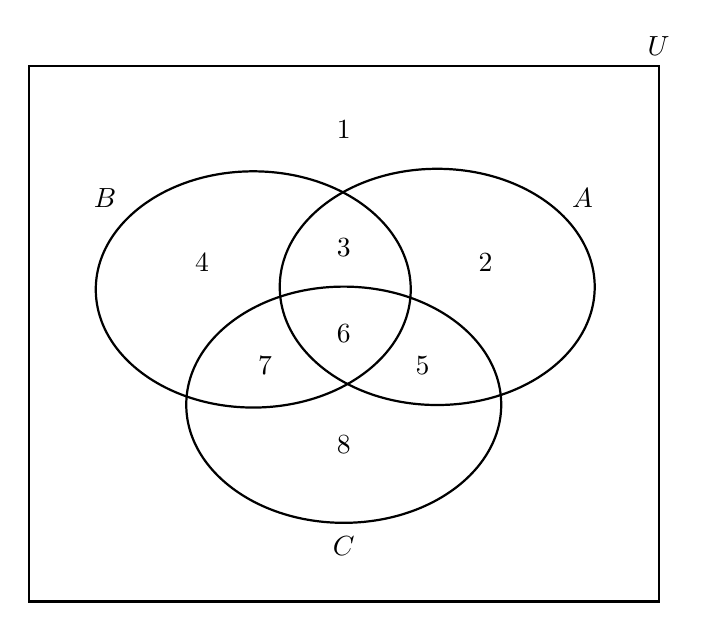
\begin{tikzpicture}[thick]
\draw (-4,-3) rectangle (4,3.8) node [above] {$U$};
\draw \firstellipse node at (35:3.7cm) {$A$};
\draw \secondellipse node at (145:3.7cm) {$B$};
\draw \thirdellipse node at (270:2.3cm) {$C$};
\node at (0,3) {1};
\node at (1.8,1.3) {2};
\node at (0,1.5) {3};
\node at (-1.8,1.3) {4};
\node at (1,0) {5};
\node at (0,0.4) {6};
\node at (-1,0) {7};
\node at (0,-1) {8};
\end{tikzpicture}

% Figuur geen veel-op-een relatie
\begin{tikzpicture}[thick]
\draw \grvertellipl node [above=3.3cm, left] {$A$};
\draw \grvertellipr node [above=3.3cm, left] {$B$};
% rechtse elementen
\draw[fill] (4,2) \bol node [above] {a};
\draw[fill] (4,0) \bol node [above] {g};
\draw[fill] (4,-2) \bol node [above] {r};
% linkse elementen
\draw[fill] (0,2) \bol node [above] {rood};
\draw[fill] (0,0) \bol node [above] {oranje};
\draw[fill] (0,-2) \bol node [above] {geel};
% pijlen
\begin{scope}[decoration={
    markings,
    mark=at position 0.5 with {\arrow{>}}}
    ] 
    \draw[postaction={decorate}] (0,2) to (4,-2);
    \draw[postaction={decorate}] (0,0) to (4,2);
    \draw[postaction={decorate}] (0,0) to (4,-2);
    \draw[postaction={decorate}] (0,-2) to (4,0);
\end{scope}
\end{tikzpicture}

% reclame-uitgaven
\begin{figure}[htbp]
    \centering
\begin{tikzpicture}[x=1cm,y=2cm]
%\draw[help lines] (0,0) grid [xstep=1, ystep=5] (8.5,3.5);
\draw[->] (-0.2,0) -- (8.2,0) node[right] {jaar na 2000};
\draw[->] (0,-0.2) -- (0,3.2) node[above] {Reclame-investeringen};
\foreach \x in {1,...,8}
	\draw[shift={(\x,0)}] (0pt,2pt) -- (0pt,-2pt) node[below] {\footnotesize $\x$};
\foreach \y in {0.5,1,...,3}
	\draw[shift={(0,\y)},color=black] (2pt,0pt) -- (-2pt,0pt) node[left] {\footnotesize $\y$};
\node [below left] at (0,0) {\footnotesize 0};
\filldraw [red] (1,1.752) circle (2pt);
\filldraw [red] (2,1.933) circle (2pt);
\filldraw [red] (3,2.137) circle (2pt) ;
\filldraw [red] (4,2.299) circle (2pt);
\filldraw [red] (5,2.387) circle (2pt);
\filldraw [red] (6,2.863) circle (2pt);
\filldraw [red] (7,3.089) circle (2pt);
\filldraw [red] (8,3.148) circle (2pt);
\end{tikzpicture}
\caption{Prijs $P(x)$}
    \label{fig:taxirecht}
\end{figure}